\documentclass[11pt]{article}
\usepackage{upquote}
\usepackage{minted}
\fvset{frame=single}

\usepackage[colorlinks=true]{hyperref}
\usepackage[margin=1in]{geometry}
\usepackage{ifthen}
\usepackage{fancyvrb}

\usepackage{listings}
\usepackage{color}

\definecolor{dkgreen}{rgb}{0,0.6,0}
\definecolor{gray}{rgb}{0.5,0.5,0.5}
\definecolor{mauve}{rgb}{0.58,0,0.82}

\lstset{frame=tb,
  language=Java,
  aboveskip=3mm,
  belowskip=3mm,
  showstringspaces=false,
  columns=flexible,
  basicstyle={\small\ttfamily},
  numbers=none,
  numberstyle=\tiny\color{gray},
  keywordstyle=\color{blue},
  commentstyle=\color{dkgreen},
  stringstyle=\color{mauve},
  breaklines=true,
  breakatwhitespace=true,
  tabsize=3
}

\usepackage{graphicx}
\usepackage{float}

\usepackage{amsmath}
\usepackage{amsfonts}
\usepackage{mathtools}

\usepackage{multirow}
\usepackage{enumitem}

\usepackage{comment}
\usepackage[usenames,dvipsnames,svgnames,table,hyperref]{xcolor}

\newcommand{\vect}[1]{\boldsymbol{#1}}
\newcommand{\matr}[1]{\boldsymbol{#1}}
\DeclareMathOperator*{\argmin}{arg\,min}
\DeclareMathOperator*{\argmax}{arg\,max}
\newcommand{\sol}[1]{{\bf{\color{magenta}{{Solution:}}}}}

\parfillskip=3em plus1fil

\title{CM146, Winter 2023 \\ Problem Set 3: Deep Learning, Learning Theory, Kernels}
\begin{document}

\author{}
\date{}
\vspace{0in}
\maketitle
\vspace{-0.75in}

\section{VC Dimension}

\subsection{(a)}
\sol x Refer to attached handwritten solutions at the end of this document.

\subsection{(b)(i)}
\sol x True. Let's assume that $V C\left(H_1\right)=d$.  This implies that there is a group of $d$ points that is shattered by $H_1$ (i.e., for any labeling of the $d$ points, there is a hypothesis $h \in H_1$ that correctly classifies them). Now, since $\mathrm{H}_2$ contains all hypotheses in $\mathrm{H}_1$, then $\mathrm{H}_2$ shatters the same set. Resultantly, we can conclude that $V C\left(H_2\right) \geq d=V C\left(H_1\right)$.

\subsection{(b)(ii)}
\sol x False. Here is a counterexample: let $H_1=\left\{h_1\right\}, H_2=\left\{h_2\right\}$, and $\forall x, h_1(x)=0, h_2(x)=1$. In this case, $V C\left(H_1\right)=V C\left(H_2\right)=0$, but $V C\left(H_1 \cup H_2\right)=1$, which disproves the given statement.

\section{Kernels}

\subsection{(a)}
\sol x $k(\mathbf{x}, \mathbf{z})$ is a kernel function. This is because we can represent it with the following matrix (which we will show is positive semi-definite). By Mercer's theorem, $k$ is a kernel function.

$$
\mathbf{K}=\left[\begin{array}{cc}
\|\mathbf{x} \cap \mathbf{x}\| & \|\mathbf{x} \cap \mathbf{z}\| \\
\|\mathbf{z} \cap \mathbf{x}\| & \|\mathbf{z} \cap \mathbf{z}\|
\end{array}\right]
$$

Since $\|\mathbf{a} \cap \mathbf{a}\|=\|\mathbf{a}\|$ for any $\mathbf{a}$ and $\|\mathbf{x} \cap \mathbf{z}\|=\|\mathbf{z} \cap \mathbf{x}\|$, $\mathbf{K}$ reduces to:

$$
\mathbf{K}=\left[\begin{array}{cc}
\|\mathbf{x}\| & \|\mathbf{x} \cap \mathbf{z}\| \\
\|\mathbf{x} \cap \mathbf{z}\| & \|\mathbf{z}\|
\end{array}\right]
$$

Now, the eigenvalues $\lambda$ of $\mathbf{K}$ are given by:

$$
\begin{gathered}
0=(\|\mathbf{x}\|-\lambda)(\|\mathbf{z}\|-\lambda)-\|\mathbf{x} \cap \mathbf{z}\|^{2} \\
\|\mathbf{x}\|\|\mathbf{z}\|-\lambda\|\mathbf{z}\|-\lambda\|\mathbf{x}\|+\lambda^{2}-\|\mathbf{x} \cap \mathbf{z}\|^{2}=0 \\
\lambda^{2}-\lambda(\|\mathbf{x}\|+\|\mathbf{z}\|)+\|\mathbf{x}\|\|\mathbf{z}\|-\|\mathbf{x} \cap \mathbf{z}\|^{2}=0
\end{gathered}
$$

Employing the property of intersections, we get $\|\mathbf{x} \cap \mathbf{z}\| \leq\|\mathbf{x}\|$ and $\|\mathbf{x} \cap \mathbf{z}\| \leq\|\mathbf{z}\|$. Hence,

$$
\|\mathbf{x} \cap \mathbf{z}\|^{2} \leq\|\mathbf{x}\|\|\mathbf{z}\|
$$

Using the quadratic formula to find the values of $\lambda$, we have:

$$
\begin{gathered}
\lambda=\frac{-(-(\|\mathbf{x}\|+\|\mathbf{z}\|)) \pm \sqrt{(-(\|\mathbf{x}\|+\|\mathbf{z}\|))^{2}-4(1)\left(\|\mathbf{x}\|\|\mathbf{z}\|-\|\mathbf{x} \cap \mathbf{z}\|^{2}\right)}}{2(1)} \\
\lambda=\frac{(\|\mathbf{x}\|+\|\mathbf{z}\|) \pm \sqrt{(\|\mathbf{x}\|+\|\mathbf{z}\|)^{2}-4\|\mathbf{x}\|\|\mathbf{z}\|+4\|\mathbf{x} \cap \mathbf{z}\|^{2}}}{2(1)}
\end{gathered}
$$

For the positive root case, $\lambda$ is trivially non-negative. For the negative case, however, we need to show that:

$$
(\|\mathbf{x}\|+\|\mathbf{z}\|)-\sqrt{(\|\mathbf{x}\|+\|\mathbf{z}\|)^{2}-4\|\mathbf{x}\|\|\mathbf{z}\|+4\|\mathbf{x} \cap \mathbf{z}\|^{2}} \geq 0
$$

Upon some rearrangement and simplification, we obtain:

$$
\begin{aligned}
(\|\mathbf{x}\|+\|\mathbf{z}\|)^{2} \geq & (\|\mathbf{x}\|+\|\mathbf{z}\|)^{2}-4\|\mathbf{x}\|\|\mathbf{z}\|+4\|\mathbf{x} \cap \mathbf{z}\|^{2} \\
& 4\|\mathbf{x}\|\|\mathbf{z}\| \geq 4\|\mathbf{x} \cap \mathbf{z}\|^{2} \\
& \|\mathbf{x}\|\|\mathbf{z}\| \geq\|\mathbf{x} \cap \mathbf{z}\|^{2}
\end{aligned}
$$

Using the equation we obtained by employing the property of intersection, this last inequality is true. Generally, we can extend this to prove that any kernel matrix is PSD. Therefore, all eigenvalues of $\mathbf{K}$ are non-negative. This means that $\mathbf{K}$ is positive semi-definite, and thus by the Mercer theorem, we can infer $k$ is a kernel function. 

\subsection{(b)}
\sol x We're given that $\mathbf{x} \cdot \mathbf{z}$ is a kernel. Using the scaling property, $k^{\prime}$ is also a kernel, where:

$$
k^{\prime}(\mathbf{x}, \mathbf{z})=\frac{\mathbf{x} \cdot \mathbf{z}}{\|\mathbf{x}\|\|\mathbf{z}\|}
$$

In this case, the scaling constants are $\|\mathbf{x}\|^{-1}$ and $\|\mathbf{z}\|^{-1}$, both of which are nonnegative. Because 1 is a kernel function (a possible generating function would be $\phi(\mathbf{x})=1$ ), by the sum property, we can conclude $1+k^{\prime}$ is also a kernel. By repeated application of the product property:

$$
\left(1+\frac{\mathbf{x}}{\|\mathbf{x}\|} \frac{\mathbf{z}}{\|\mathbf{z}\|}\right)^{3}=\left(1+k^{\prime}\right)^{3}=\left(1+k^{\prime}\right)\left(1+k^{\prime}\right)\left(1+k^{\prime}\right) \\
$$

Hence, this is also a kernel.

\subsection{(c)}
\sol x We can begin by defining the kernel $k_{\beta}(\mathbf{x}, \mathbf{z})=(1+\beta \mathbf{x} \cdot \mathbf{z})^{3}$, and expanding it:

$$
\begin{gathered}
1+3 \beta \mathbf{x} \cdot \mathbf{z}+3 \beta^{2}(\mathbf{x} \cdot \mathbf{z})^{2}+\beta^{3}(\mathbf{x} \cdot \mathbf{z})^{3} \\
1+3 \beta x_{1} z_{1}+3 \beta x_{2} z_{2}+3 \beta^{2}\left(x_{1}^{2} z_{1}^{2}+2 x_{1} x_{2} z_{1} z_{2}+x_{2}^{2} z_{2}^{2}\right)+\beta^{3}\left(x_{1}^{3} x_{2}^{3}+3 x_{1}^{2} x_{2}^{2} z_{1} z_{2}+3 x_{1} x_{2} z_{1}^{2} z_{2}^{2}+z_{1}^{3} z_{2}^{3}\right)
\end{gathered}
$$

Our intention to find a function $\phi$ such that $\phi(\mathbf{x})^{\mathrm{T}} \phi(\mathbf{z})$ equals the expression above. Using a method similar to the case for 2nd-degree polynomials, we get:

$$
\phi=\left[\begin{array}{c}
1 \\
\sqrt{3 \beta} x_{1} \\
\sqrt{3 \beta} x_{2} \\
\sqrt{3} \beta x_{1}^{2} \\
\sqrt{3} \beta x_{2}^{2} \\
\sqrt{6} \beta x_{1} x_{2} \\
\sqrt{\beta^{3}} x_{1}^{3} \\
\sqrt{\beta^{3}} x_{2}^{3} \\
\sqrt{3 \beta^{3}} x_{1}^{2} x_{2} \\
\sqrt{3 \beta^{3}} x_{1} x_{2}^{2}
\end{array}\right]
$$

Both methods involve computing the dot product of vectors $\mathbf{x}$ and $\mathbf{z}$. However, in the case of the kernel function $k(\mathbf{x}, \mathbf{z})=(1+\mathbf{x} \cdot \mathbf{z})^{3}$, the scaling factor $\beta$ is absent for each term when $\beta=1$. As the degree of the transformation vector increases, the scaling factor $\beta$ also increases, which may be utilized as a regularization parameter.

\section{SVM}

\subsection{(a)}
\sol x To solve this, we can use Lagrange multipliers. In this case,

$$
f(\boldsymbol{\theta})=\frac{1}{2}\|\boldsymbol{\theta}\|^{2} \text { and } g(\boldsymbol{\theta})=y_{n} \boldsymbol{\theta}^{T} \mathbf{x}_{n} \geq 1
$$

For a training vector $x=\left[\begin{array}{ll}a & e\end{array}\right]^{T}$ with label $y=-1$, we can reduce this to:

$$
f(\boldsymbol{\theta})=\frac{1}{2}\|\boldsymbol{\theta}\|^{2} \text { and } g(\boldsymbol{\theta})=-\boldsymbol{\theta}^{T} \mathbf{x}_{n} \geq 1
$$

The Lagrangian is

$$
L=\frac{1}{2}\|\boldsymbol{\theta}\|^{2}-\lambda\left(-\boldsymbol{\theta}^{T} \mathbf{x}_{n}-1\right)=\frac{1}{2}\|\boldsymbol{\theta}\|^{2}+\lambda\left(\boldsymbol{\theta}^{T} \mathbf{x}_{n}+1\right)
$$

Since there's a requirement to minimize this over $\boldsymbol{\theta}$, we take the derivative with respect to it, and set it to 0:

$$
\begin{gathered}
\frac{\partial L}{\partial \boldsymbol{\theta}}=\boldsymbol{\theta}+\lambda \mathbf{x}_{n}=0 \\
\boldsymbol{\theta}^{*}=-\lambda \mathbf{x}_{n}
\end{gathered}
$$

Now, to maximize $\lambda$, we can substitute in the previous result, take the derivative with respect to $\lambda$, and set it to 0:

$$
\begin{gathered}
L=\frac{1}{2}\left\|-\lambda \mathbf{x}_{n}\right\|^{2}+\lambda\left(\left(-\lambda \mathbf{x}_{n}\right)^{T} \mathbf{x}_{n}+1\right) \\
L=\frac{1}{2} \lambda^{2}\left\|\mathbf{x}_{n}\right\|^{2}-\lambda^{2}\left\|\mathbf{x}_{n}\right\|^{2}+\lambda=-\frac{1}{2} \lambda^{2}\left\|\mathbf{x}_{n}\right\|^{2}+\lambda \\
\frac{\partial L}{\partial \lambda}=-\lambda\left\|\mathbf{x}_{n}\right\|^{2}+1=0 \\
\lambda^{*}=\frac{1}{\left\|\mathbf{x}_{n}\right\|^{2}}
\end{gathered}
$$

Lastly, we can substitute this $\lambda^{*}$ value into the expression for $\theta^{*}$ to obtain a value that satisfies the given constrained minimization:

$$
\begin{gathered}
\boldsymbol{\theta}^{*}=-\frac{1}{\left\|\mathbf{x}_{n}\right\|} \mathbf{x}_{n} \\
\boldsymbol{\theta}^{*}=-\frac{1}{a^{2}+e^{2}}\left[\begin{array}{l}
a \\
e
\end{array}\right]
\end{gathered}
$$

\subsection{(b)}
\sol x This optimization problem can be written as follows:

$$
\begin{gathered}
f(\boldsymbol{\theta})=\frac{1}{2}\|\boldsymbol{\theta}\|^{2} \\
g_{1}(\boldsymbol{\theta})=\boldsymbol{\theta}^{T} \mathbf{x}_{1} \geq 1 \\
g_{2}(\boldsymbol{\theta})=\boldsymbol{\theta}^{T} \mathbf{x}_{2} \leq-1
\end{gathered}
$$

Assuming the data has 2 dimensions, the two constraint equations give

$$
\theta_{1}+\theta_{2} \geq 1 \text { and } \theta_{1} \leq-1
$$

The goal is to minimize the magnitude of $\boldsymbol{\theta}$, so we pick the value $\theta_{2}=-1$, which gives $\theta_{1}=2$. The margin in this case is $\frac{1}{\|\boldsymbol{\theta}\|_{2}}=\frac{\sqrt{5}}{5}$. This gives us the answer:

$$
\theta^{*}=\left[\begin{array}{c}
-1 \\
2
\end{array}\right] \text { and } \gamma=\frac{\sqrt{5}}{5}
$$

\subsection{(c)}
\sol x Since $b$ is allowed to be nonzero, the constraint equations become:

$$
\theta_{1}+\theta_{2}+b \geq 1 \text { and } \theta_{1}+b \leq-1
$$

Then, to minimize the magnitude of $\boldsymbol{\theta}$, we can set $b=-1$ so that $\theta_{2}=0$, and then $\theta_{1}+0-1 \geq 1$, giving $\theta_{1}=2$. Resultantly, the new values are

$$
\left(\boldsymbol{\theta}^{*}, b^{*}\right)=\left(\left[\begin{array}{ll}
1 & 0
\end{array}\right]^{\mathrm{T}},-1\right) \text {, and } \gamma=0.5
$$

The magnitude of $\boldsymbol{\theta}$ has decreased, while the margin has increased. This makes sense because we are now allowing a greater set of hyperplanes to pick from, so the classifier is able to find a better one with smaller magnitude of $\boldsymbol{\theta}$ and a larger margin. 

\section{Implementation: Digit Recognizer}
\subsection{Data Visualization and Preparation}

\subsubsection*{(a)}
\sol x 
\begin{lstlisting}
    plot_img(X_train[5])
    plot_img(X_train[6])
    plot_img(X_train[7])
\end{lstlisting}

\begin{center}
    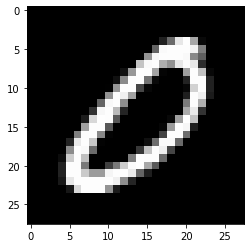
\includegraphics[scale=0.5]{4a-1.png} \\
    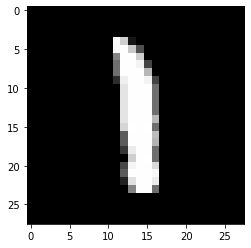
\includegraphics[scale=0.5]{4a-2.png} \\
    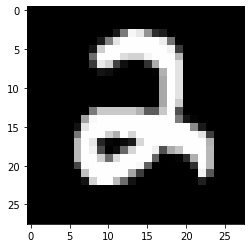
\includegraphics[scale=0.5]{4a-3.png} \\
\end{center}

\subsubsection*{(b)}
\sol x 
\begin{lstlisting}
    X_train = torch.from_numpy(X_train)
    y_train = torch.from_numpy(y_train)
    X_valid = torch.from_numpy(X_valid)
    y_valid = torch.from_numpy(y_valid)
    X_test = torch.from_numpy(X_test)
    y_test = torch.from_numpy(y_test)
\end{lstlisting}

\subsubsection*{(c)}
\sol x 
\begin{lstlisting}
    train_data = TensorDataset(X_train,y_train)
    valid_data = TensorDataset(X_valid,y_valid)
    test_data = TensorDataset(X_test,y_test)
    train_loader = DataLoader(train_data, shuffle=True, batch_size=10)
    valid_loader = DataLoader(valid_data, shuffle=False, batch_size=10)     
    test_loader = DataLoader(test_data, shuffle=False, batch_size=10)
\end{lstlisting}

\subsection{One-Layer Network}

\subsubsection*{(d)}
\sol x 
\begin{lstlisting}
class OneLayerNetwork(torch.nn.Module):
    def __init__(self):
        super(OneLayerNetwork, self).__init__()
        
        ### ========== TODO : START ========== ###
        ### part d: implement OneLayerNetwork with torch.nn.Linear 
        self.linear = torch.nn.Linear(784, 3)
        ### ========== TODO : END ========== ###
    
    def forward(self, x):
        # x.shape = (n_batch, n_features)
        ### ========== TODO : START ========== ### 
        ### part d: implement the forward function 
        outputs = self.linear(x)
        ### ========== TODO : END ========== ### 
        return outputs
\end{lstlisting}

\subsubsection*{(e)}
\sol x 
\begin{lstlisting}
    ### ========== TODO : START ========== ###
    ### part e: prepare OneLayerNetwork, criterion, and optimizer
    model_one = OneLayerNetwork()
    criterion = torch.nn.CrossEntropyLoss()
    optimizer = torch.optim.SGD(model_one.parameters(), lr=0.0005)
    ### ========== TODO : END ========== ###
\end{lstlisting}

\subsubsection*{(f)}
\sol x 
\begin{lstlisting}
    ### ========== TODO : START ========== ###
    ### part f: implement the training process
    pred = model.forward(batch_X)
    optimizer.zero_grad()
    loss = criterion(pred, batch_y)
    loss.backward()
    optimizer.step()
    ### ========== TODO : END ========== ###
\end{lstlisting}

\subsection{Two-Layer Network}

\subsubsection*{(g)}
\sol x 
\begin{lstlisting}
class TwoLayerNetwork(torch.nn.Module):
    def __init__(self):
        super(TwoLayerNetwork, self).__init__()
        ### ========== TODO : START ========== ###
        ### part g: implement TwoLayerNetwork with torch.nn.Linear
        self.hidden = torch.nn.Linear(784, 400)
        self.output = torch.nn.Linear(400, 3)
        ### ========== TODO : END ========== ###

    def forward(self, x):
        # x.shape = (n_batch, n_features)

        ### ========== TODO : START ========== ###
        ### part g: implement the foward function
        hidden = self.hidden(x)
        hidden = torch.nn.sigmoid(hidden)
        outputs = self.output(hidden)
        ### ========== TODO : END ========== ###
        return outputs
\end{lstlisting}

\subsubsection*{(h)}
\sol x 
\begin{lstlisting}
    ### ========== TODO : START ========== ###
    ### part h: prepare TwoLayerNetwork, criterion, and optimizer
    model_two = TwoLayerNetwork()
    criterion = torch.nn.CrossEntropyLoss()
    optimizer =  torch.optim.SGD(model_two.parameters(), lr=0.0005)
    ### ========== TODO : END ========== ###
\end{lstlisting}

\subsection{Performance Comparison}

\subsubsection*{(i)}
\sol x The rate of decrease in loss for the training and validation set is much slower in the two-layered model compared to the one-layered network. The reason for this slow learning is that in the two-layered network, the error gradient is back-propagated through the network with each adjustment. This back-propagation uses the chain rule, which can result in very small derivatives that barely change the weights in the initial layers when adjustments are made. The one-layer network has fewer parameters, making optimization easier and faster convergence possible. Additionally, both models have similar training and validation loss, indicating good generalization and no overfitting. \\

\begin{lstlisting}
    ### ========== TODO : START ========== ###
    ### part i: generate a plot to comare one_train_loss, one_valid_loss, two_train_loss, two_valid_loss
    epochs = range(1, len(one_train_loss) + 1)
    plt.plot(epochs, one_train_loss, linestyle='.', label='Model 1 Training Loss')
    plt.plot(epochs, one_valid_loss, linestyle='.', label='Model 1 Validation Loss')
    plt.plot(epochs, two_train_loss, linestyle='.', label='Model 2 Training Loss')
    plt.plot(epochs, two_valid_loss, linestyle='.', label='Model 2 Validation Loss')
    plt.xlabel('Epoch')
    plt.ylabel('Loss')
    plt.title('Loss vs. Epochs')
    plt.legend()
    plt.show()
    ### ========== TODO : END ========== ###
\end{lstlisting}

\begin{center}
    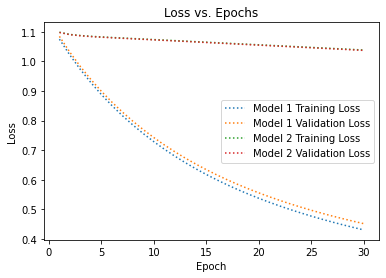
\includegraphics[scale=0.6]{4i.png} \\
\end{center}


\subsubsection*{(j)}
\sol x The graph indicates that the one-layer neural network is currently performing better than the two-layer neural network in terms of convergence. The two-layered neural network has a slower growth in accuracy due to having more weights to change and back-propagating through them, which results in small derivatives that adjust the weights slowly. However, the accuracies of both models become similar in the later epochs. It's worth noting that the accuracy on the validation dataset is consistently lower than the accuracy on the training dataset, indicating slight potential overfitting. Nevertheless, the data generalizes well since the difference is not significant. The one-layer model has train and validation accuracies around 95\%, while the two-layer model has train and validation accuracies around 88\%. \\

\begin{lstlisting}
    ### ========== TODO : START ========== ###
    ### part j: generate a plot to comare one_train_acc, one_valid_acc, two_train_acc, two_valid_acc
    epochs = range(1, len(one_train_acc) + 1)
    plt.plot(epochs, one_train_acc, linestyle='.', label='Model 1 Training Accuracy')
    plt.plot(epochs, one_valid_acc, linestyle='.', label='Model 1 Validation Accuracy')
    plt.plot(epochs, two_train_acc, linestyle='.', label='Model 2 Training Accuracy')
    plt.plot(epochs, two_valid_acc, linestyle='.', label='Model 2 Validation Accuracy')
    plt.xlabel('Epoch')
    plt.ylabel('Accuracy')
    plt.title('Accuracy vs. Epochs')
    plt.legend()
    plt.show()
    ### ========== TODO : END ========== ##
\end{lstlisting}

\begin{center}
    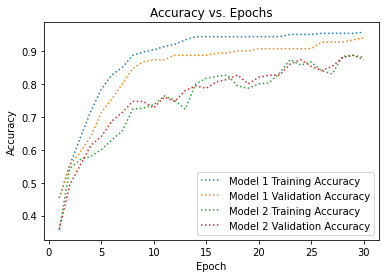
\includegraphics[scale=0.6]{4j.png} \\
\end{center}

 \subsubsection*{(k)}
\sol x \\
\\
One-Layer Network Test Accuracy: 96.00\% \\
Two-Layer Network Test Accuracy: 84.67\% \\

The test accuracy of the one-layer network is considerably better than that of the two-layer network, which can be attributed to two possible reasons. Firstly, since the two-layer network has more parameters, it may require a longer training process than the 30 epochs provided in the experiment. Secondly, it's possible that the two-layer network overfitted, but the accuracy vs. epoch graph suggests that any such effect, if present, is insignificant. \\

\begin{lstlisting}
    ### ========== TODO : START ========== ###
    ### part k: calculate the test accuracy
    m1_acc = evaluate_acc(model_one, test_loader)
    m2_acc = evaluate_acc(model_two, test_loader)
    
    print("One Neural Net Test Accuracy:", m1_acc)
    print("Two Neural Net Test Accuracy:", m2_acc)
    print("Two Neural Net Val Acc:", two_valid_acc[29])
    ### ========== TODO : END ========== ###
\end{lstlisting}

\begin{center}
    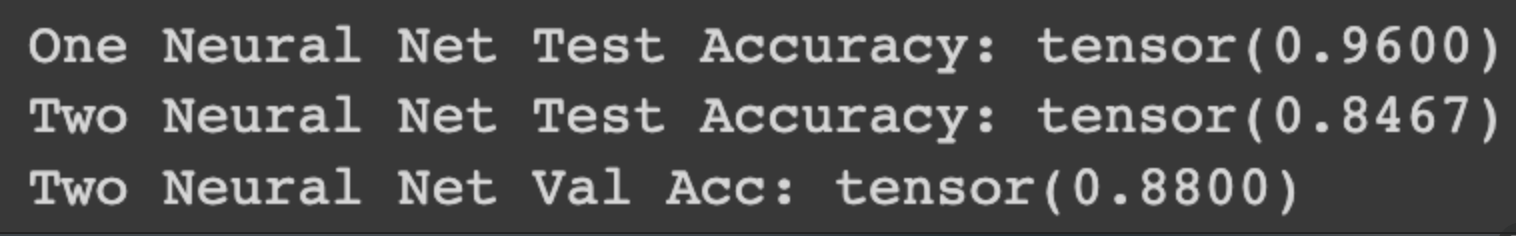
\includegraphics[scale=0.3]{4k.png} \\
\end{center}

\subsubsection*{(l)}
\sol x The Adam optimizer yields quicker convergence than the SGD optimizer, enabling us to realize the true accuracy of the two-layer network as it converges. Based on the graphs, the two-layer network performs better than the one-layer network on both training and validation data, and equally well on test data. It's evident that the Adam optimizer is superior to SGD in this scenario. The two-layer network achieves a validation accuracy of 97.5\% within five epochs. One possible explanation for the identical test accuracies of the models is the limitations imposed by the small dataset. According to learning theory, the generalization error depends on the number of training examples, and certain outliers in the test data can prevent the accuracy from reaching 100\%. Therefore, it's possible that both models have learned the maximum amount from the limited training examples, resulting in the same test accuracy. \\

\begin{center}
    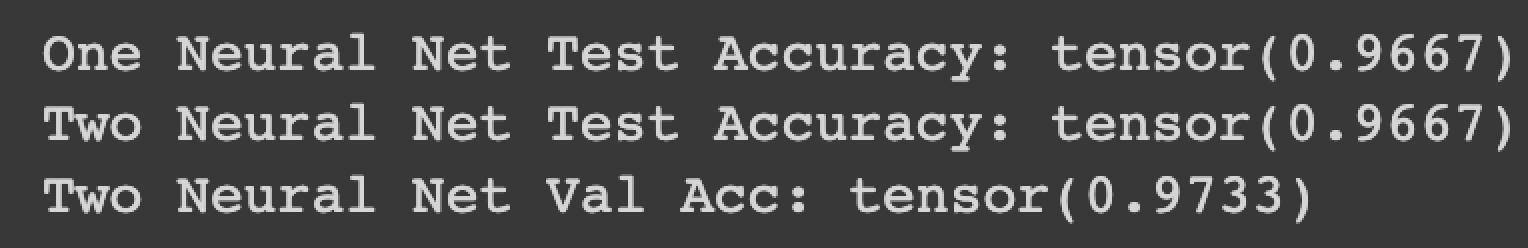
\includegraphics[scale=0.3]{4l-3.png} \\
\end{center}

\begin{lstlisting}
    optimizer = torch.optim.Adam(model_one.parameters(), lr=0.0005)
\end{lstlisting}

\begin{center}
    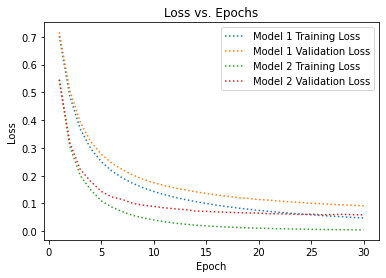
\includegraphics[scale=0.6]{4l-1.png} \\
    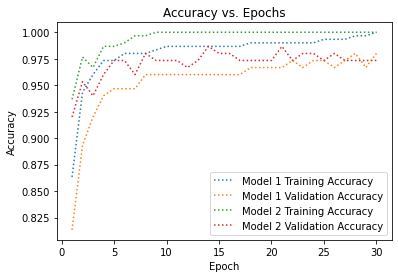
\includegraphics[scale=0.6]{4l-2.png} \\
\end{center}

\end{document}
